\PassOptionsToPackage{draft}{graphicx}

\documentclass{beamer}

\usepackage[version=4]{mhchem}  
\usepackage{tikz}
\usepackage{caption}
%\usepackage[lithuanian,english]{babel}
\usepackage{polyglossia}
\setmainlanguage{lithuanian}
\usepackage[
    backend=biber,
    style=numeric,
    sorting=ynt
]{biblatex}

\bibliography{slides/bibliografija}

\usetheme{Copenhagen}

\setbeamertemplate{caption}[numbered]

%Information to be included in the title page:
\title{Sample title}
\author{Anonymous}
\institute{Overleaf}
\date{2025}

%\section{Medžiagų maišymo modeliavimas cheminėse reakcijose}
\setbeamertemplate{headline}{}

\title[]
{Medžiagų maišymo modeliavimas cheminėse reakcijose}

\subtitle{Modelling the mixing of reagents in chemical reactions}

\author[Arnas Vaicekauskas]
{
    A.~Vaicekauskas\inst{1}\\ 
    \small Darbo vadovas: Asist. Dr. R.~Astrauskas\inst{1}
}

\institute[MIF]
{
  \inst{1}
  Matematikos ir informatikos fakultetas\\
  Vilniaus Universitetas
}


\begin{document}

\frame{\titlepage}

\begin{frame}
\frametitle{Ytrio aliuminio granatas (YAG)}

\begin{figure}
    \centering
    \begin{minipage}{.5\textwidth}
        \centering
        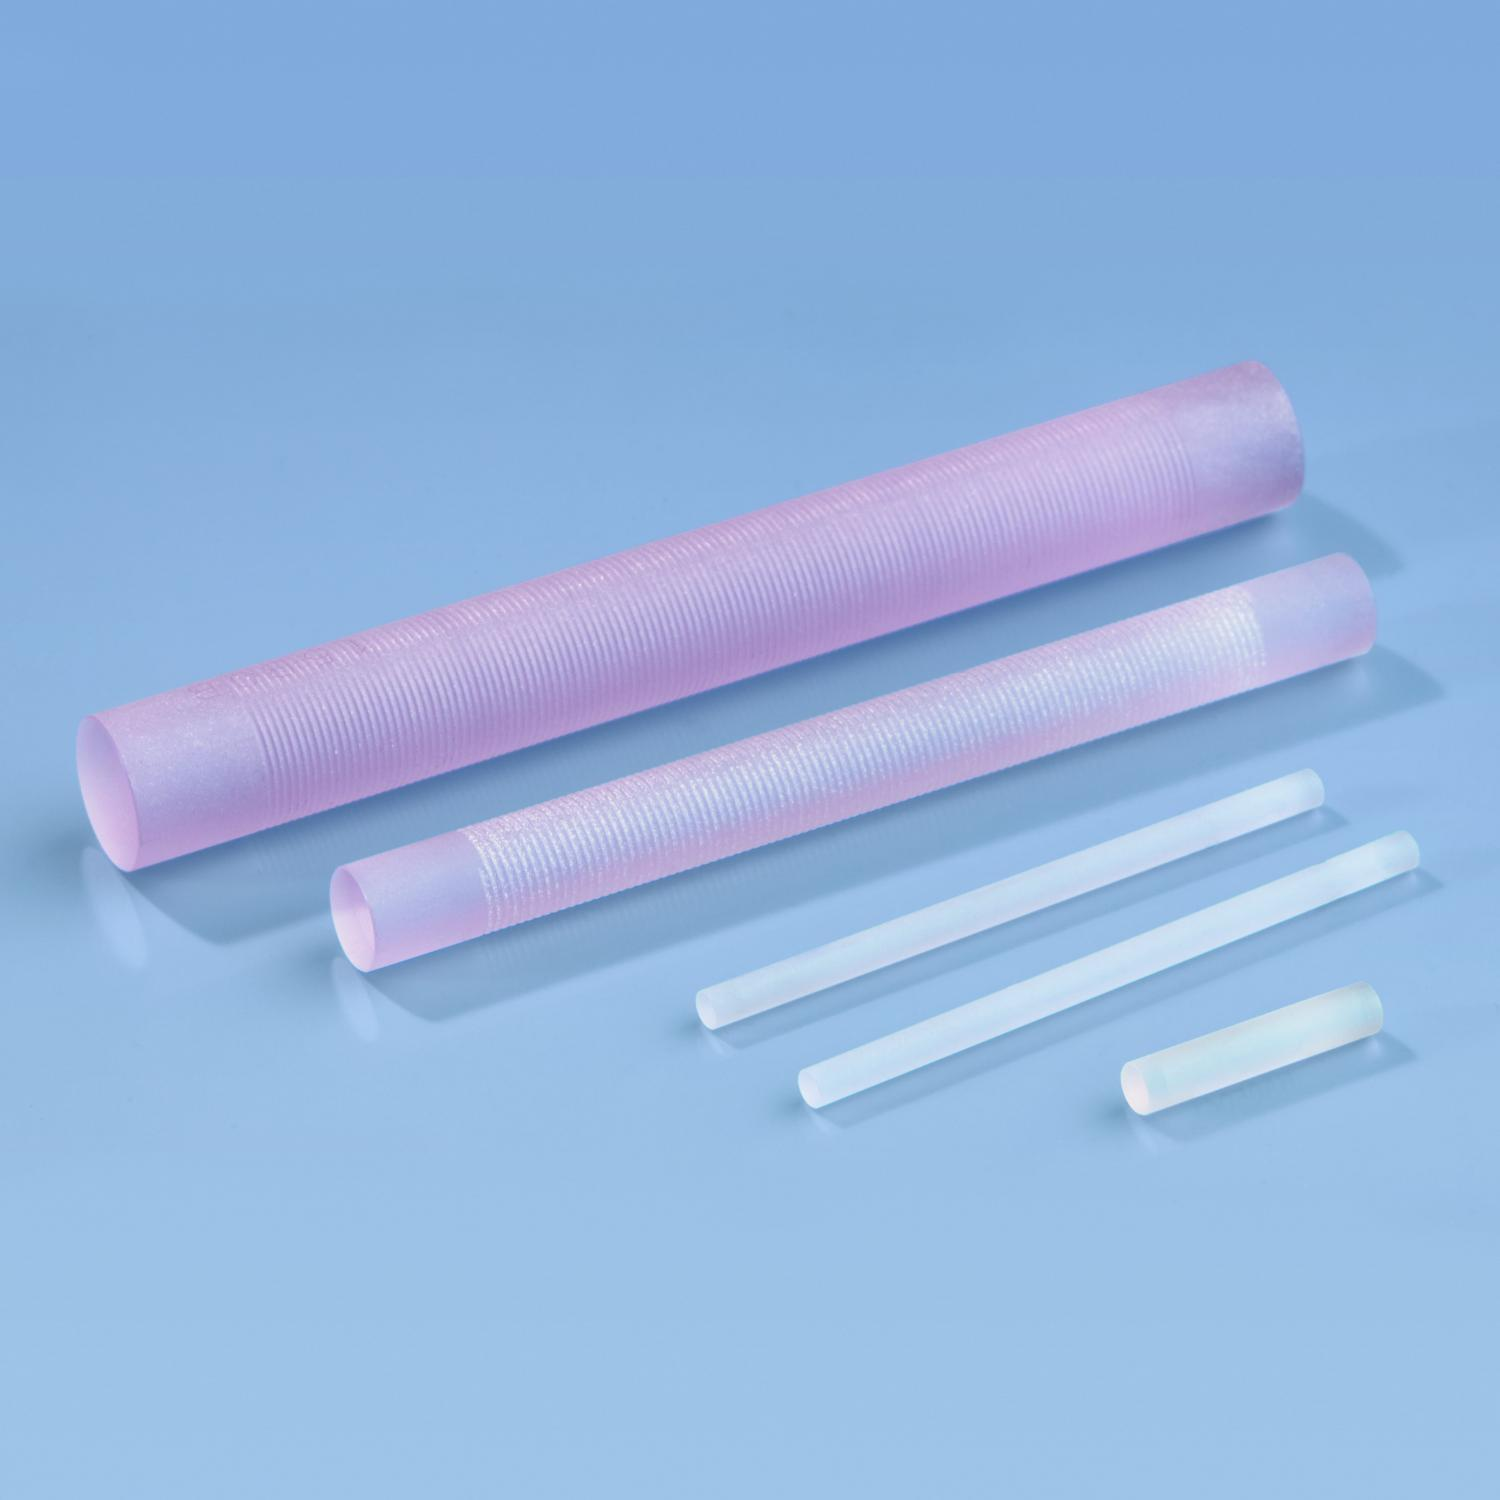
\includegraphics[width=0.8\textwidth]{../slides/assets/nd:yag.png}
        \caption{Apdoroti YAG kristalai \cite{NdYAGCrystals}}
    \end{minipage}%
    \begin{minipage}{.5\textwidth}
               
    \end{minipage}
\end{figure}

\begin{itemize}
    \item Plačiausiai naudojama medžiaga lazerių aktyviosioms terpėms gaminti
    \item YAG lazeriai naudojami medicinos bei gamybos srityse
\end{itemize}

\end{frame}

\begin{frame}
\frametitle{YAG cheminė reakcija}

\centering
\begin{align*}
    \ce{3Y_2O_3 + 5Al_2O_3 -> 2Y_3Al_5O_{12}}
\end{align*}    
\begin{itemize}
\item YAG kristalai sintezuojami kaitinant Aliuminio ir Itrio oksidų mišinį
\item Reakcija gali užtrukti keliolika valandų
\item Chemikai vykstant reakcijai periodiškai išmaišo reagentus, kad reakcijos laikas sutrumpėtų
\end{itemize}

\end{frame}

\begin{frame}
\frametitle{Darbo tikslas ir uždaviniai}
\textbf{Tikslas} - sukurti kompiuterinį YAG reakcijos maišymo modelį ir jį ištirti.

\textbf{Uždaviniai:}
\begin{enumerate}
\item Sukurti kompiuterinį YAG reakcijos modelį
\item Patikrinti kompiuterinio modelio rezultatų korektiškumą
\item Papildyti kompiuterinį modelį su maišymo procesu
\item Ištirti kompiuterinio modelio rezultatus
\end{enumerate}

\end{frame}

\begin{frame}
\frametitle{Matematinis modelis}

YAG Reakcijos--difuzijos sistema

\begin{align*}
    \frac{\partial c_1}{\partial t} & =-3kc_1c_2+D\left(\frac{\partial^2c_1}{\partial x^2}+\frac{\partial^2c_1}{\partial y^2}\right) \\
    \frac{\partial c_2}{\partial t} & =-5kc_1c_2+D\left(\frac{\partial^2c_2}{\partial x^2}+\frac{\partial^2c_2}{\partial y^2}\right)\\
    \frac{\partial c_3}{\partial t} & =2kc_1c_2\\
    (x, y, t)&\in(0, W)\times(0, H)\times[0, T]
\end{align*}

\end{frame}

\begin{frame}
    \frametitle{Pradinės ir kraštinės sąlygos}
    \begin{figure}
        \centering
        \begin{tikzpicture}[scale=2.0]
            \draw[fill=white] (0,0) rectangle (1,1);
            \draw[fill=white] (1,1) rectangle (2,2);
            \draw[fill=gray!50] (0,1) rectangle (1,2);
            \draw[fill=gray!50] (1,0) rectangle (2,1);
    
            % Draw the boundary of the square
            \draw[thick] (0,0) rectangle (2,2);
    
            % Draw axes
            \draw[->] (-0.5, 0) -- (2.5, 0) node[anchor=north west] {$x$};
            \draw[->] (0, -0.5) -- (0, 2.5) node[anchor=north east] {$y$};
    
            % Mark the origin
            \node[anchor=north east] at (0,0) {$(0, 0)$};
    
            % Mark the side length
            \draw[-] (2,0) -- (2,2);
            \draw[-] (0,2) -- (2,2);

            \node at (2.1, 0.75) {$H$};
            \node at (0.75, 2.1) {$W$};
            
            \draw (0.5, 1.5) node[anchor=center] {$5c_0$};
            \draw (1.5, 0.5) node[anchor=center] {$5c_0$};
            \draw (1.5, 1.5) node[anchor=center] {$3c_0$};
            \draw (0.5, 0.5) node[anchor=center] {$3c_0$};

            % boundary conditions
            \draw[->] (-0.05,1) -- (-0.55,1);
            \node at (-0.55, 1.5) {$\frac{dc_m}{dx} = 0$};

            \draw[->] (2.05,1) -- (2.55,1);
            \node at (2.55, 1.5) {$\frac{dc_m}{dx} = 0$};

            \draw[->] (1, -0.05) -- (1, -0.55);
            \node at (1.5, -0.25) {$\frac{dc_m}{dy} = 0$};

            \draw[->] (1, 2.05) -- (1, 2.55);
            \node at (1.5, 2.25) {$\frac{dc_m}{dy} = 0$};

        \end{tikzpicture}
        \caption{Pradinės ir kraštinės sąlygos modeliui.}
        \label{initial-boundary-condition}
    \end{figure}
\end{frame}

\begin{frame}
    \frametitle{Stabilumas}
    Galima parodyti, kad skaitinis sprendinys bus stabilus tada, kai tenkinama ši nelygybė:
    \begin{align*}
        \Delta t \leqslant \left(15kc_0+2D\left((\Delta x)^{-2}+(\Delta y)^{-2}\right)\right)^{-1}
    \end{align*}
    Čia $k$ - reakcijos greitis, $D$ - difuzijos konstanta, $\Delta x, \Delta y$ - diskretūs erdvės žingsniai, $c_0$ - pradinių medžiagų koncentracijų didžiausias bendras daliklis.
\end{frame}

\begin{frame}
    \frametitle{Reakcijos--difuzijos modelio rezultatai}
    Modelio evoliucija laike su pradinėmis ir kraštinėmis sąlygomis \eqref{initial-boundary-condition}
    \centering
    
\includegraphics[width=12cm]{paper/assets/example-0.png} \\ 
    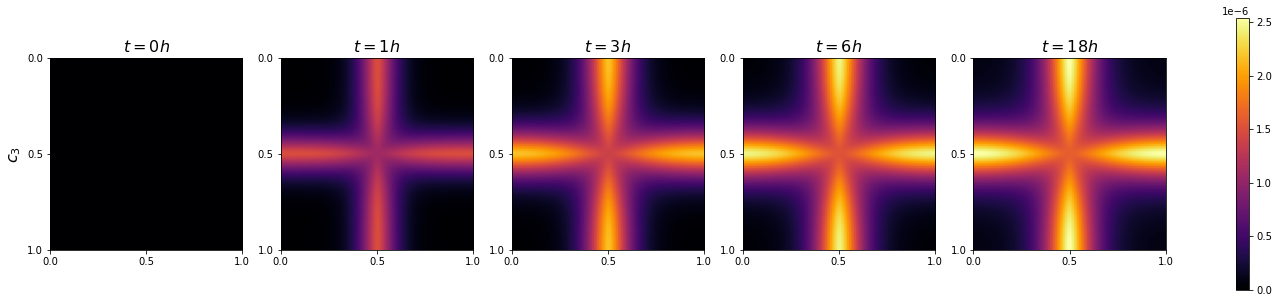
\includegraphics[width=12cm]{paper/assets/example-2.png}

\end{frame}

\begin{frame}
    \frametitle{Reakcijos stabdymo sąlyga}
    \begin{align*}
        q(t_\text{stop})=0.03q(0)
    \end{align*}
    Čia $q(t)$ yra pirmos ir antros medžiagų kiekis sistemoje. Reakcija stabdoma tada, kai pirmų dviejų medžiagų kiekis sistemoje pasiekia 3\% pradinio kiekio.
\end{frame}

\begin{frame}
\frametitle{Atsitiktinis maišymas}
\begin{figure}
\centering
\begin{tikzpicture}[scale=1.5]

    \fill[gray!30] (0,1) rectangle (1, 2);
    \fill[gray!30] (1,0) rectangle (2, 1);

    % Original Grid
    \draw[thick] (0,0) rectangle (2,2);
    \draw[thick] (1,0) -- (1,2);
    \draw[thick] (0,1) -- (2,1);

    \node at (0.5,1.5) {$\Omega_1$};
    \node at (1.5,1.5) {$\Omega_2$};
    \node at (0.5,0.5) {$\Omega_3$};
    \node at (1.5,0.5) {$\Omega_4$};

    % Arrow
    \draw[->, thick] (2.5,1) -- (3.5,1);

    % Transformed Grid
    \begin{scope}[shift={(4,0)}]

        \fill[gray!30] (0,0) rectangle (1, 1);
        \fill[gray!30] (1,1) rectangle (2, 2);

        \draw[thick] (0,0) rectangle (2,2);
        \draw[thick] (1,0) -- (1,2);
        \draw[thick] (0,1) -- (2,1);

        \node at (0.5,1.5) {\rotatebox{270}{$\Omega_3$}}; % Rotated 180° horizontally
        \node at (1.5,1.5) {$\Omega_1$};             % No change
        \node at (0.5,0.5) {\rotatebox{180}{$\Omega_4$}}; % Upside down
        \node at (1.5,0.5) {\rotatebox{90}{$\Omega_2$}};  % 90° rotation
    \end{scope}
\end{tikzpicture}
\caption{Atsitiktinio išmaišymo metu metu reakcijos erdvės sritys yra atsitiktinai pasukamos ir susikeičiamos vietomis. }
\label{random-mix}
\end{figure}
\end{frame}

\begin{frame}
    \frametitle{Atsitiktinio maišymo rezultatai}
    \begin{figure}
        \centering
        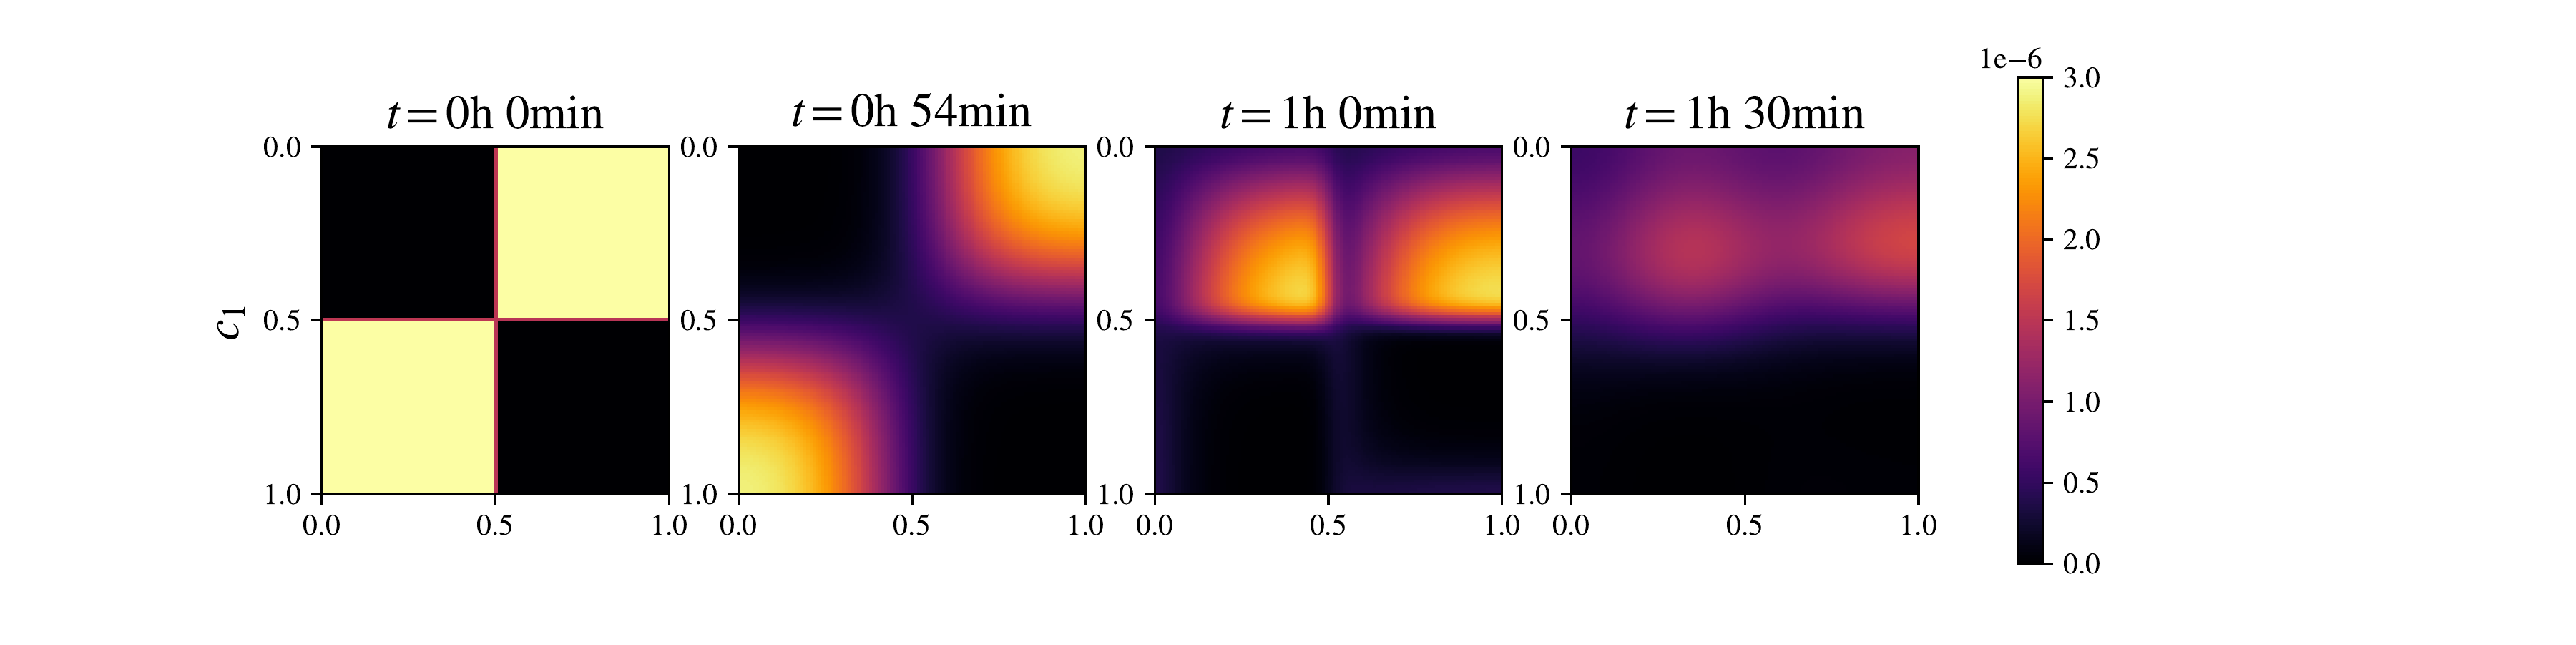
\includegraphics[width=12cm]{paper/assets/random-mix-example-c0-1.png} \\
        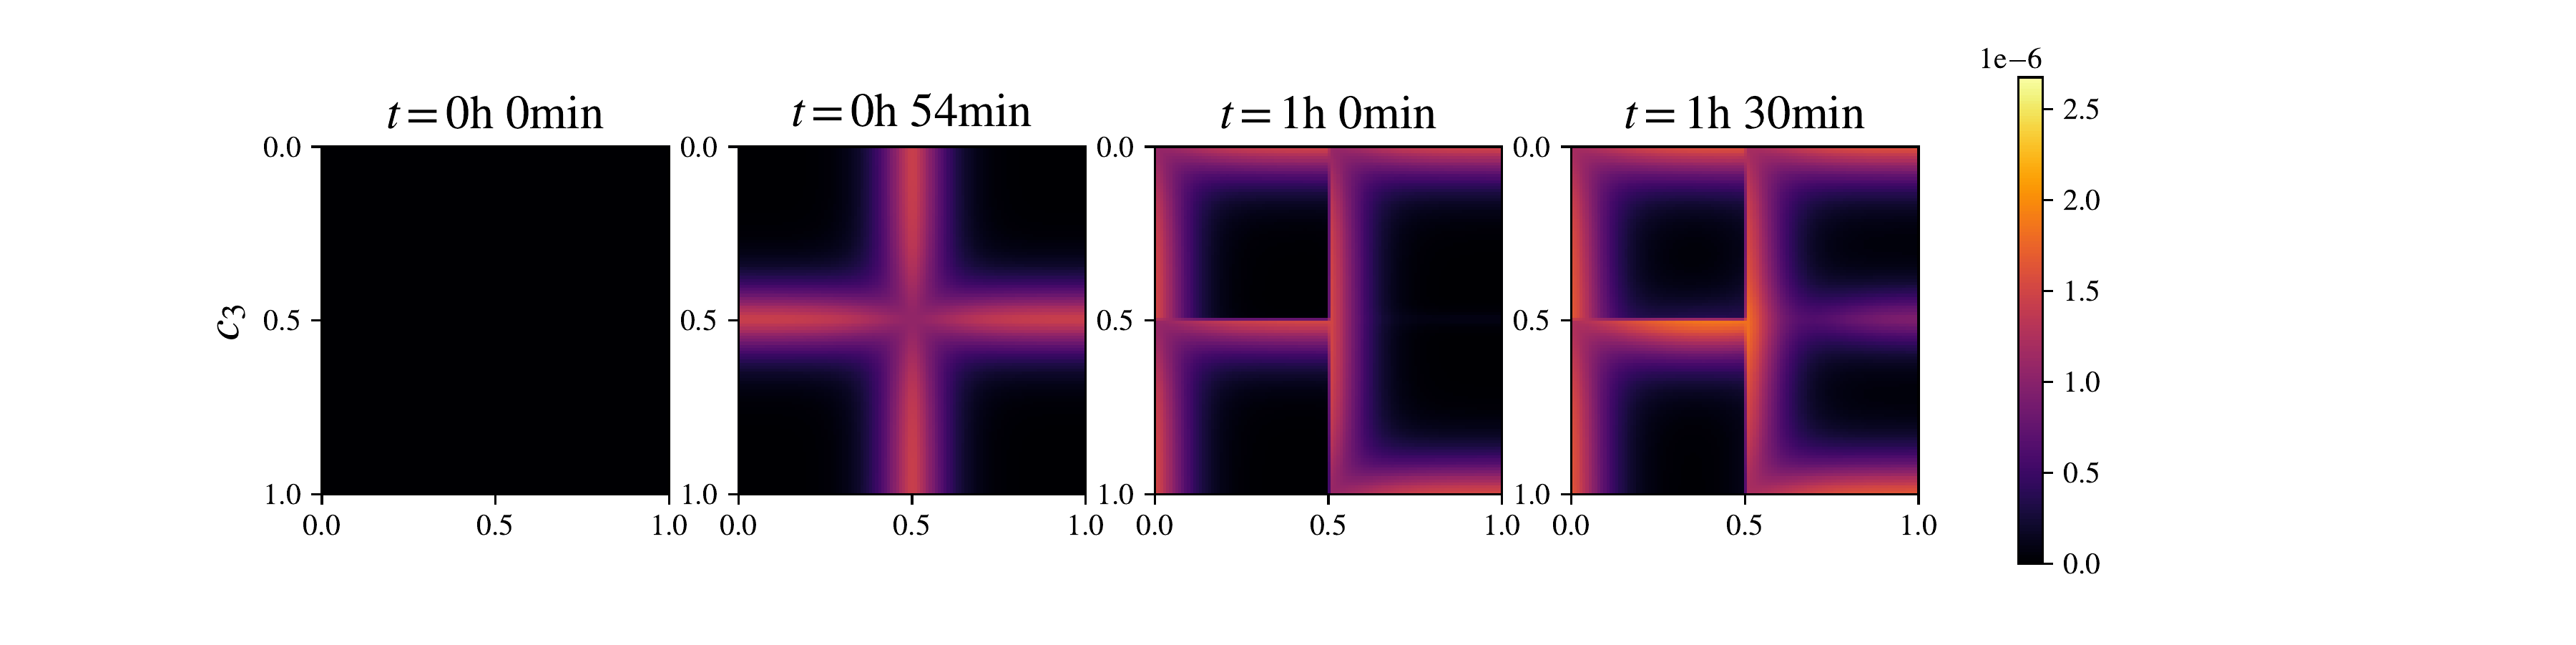
\includegraphics[width=12cm]{paper/assets/random-mix-example-c2-1.png}
        \caption{Modelio evoliucija laike su pradinėmis ir kraštinėmis sąlygomis \eqref{initial-boundary-condition}, kai naudojamas atsitiktinio išmaišymo modelis \eqref{random-mix}.}
    \end{figure}
\end{frame}

\begin{frame}
    \frametitle{Atsitiktinio maišymo rezultatai}
    \begin{figure}
        \centering
        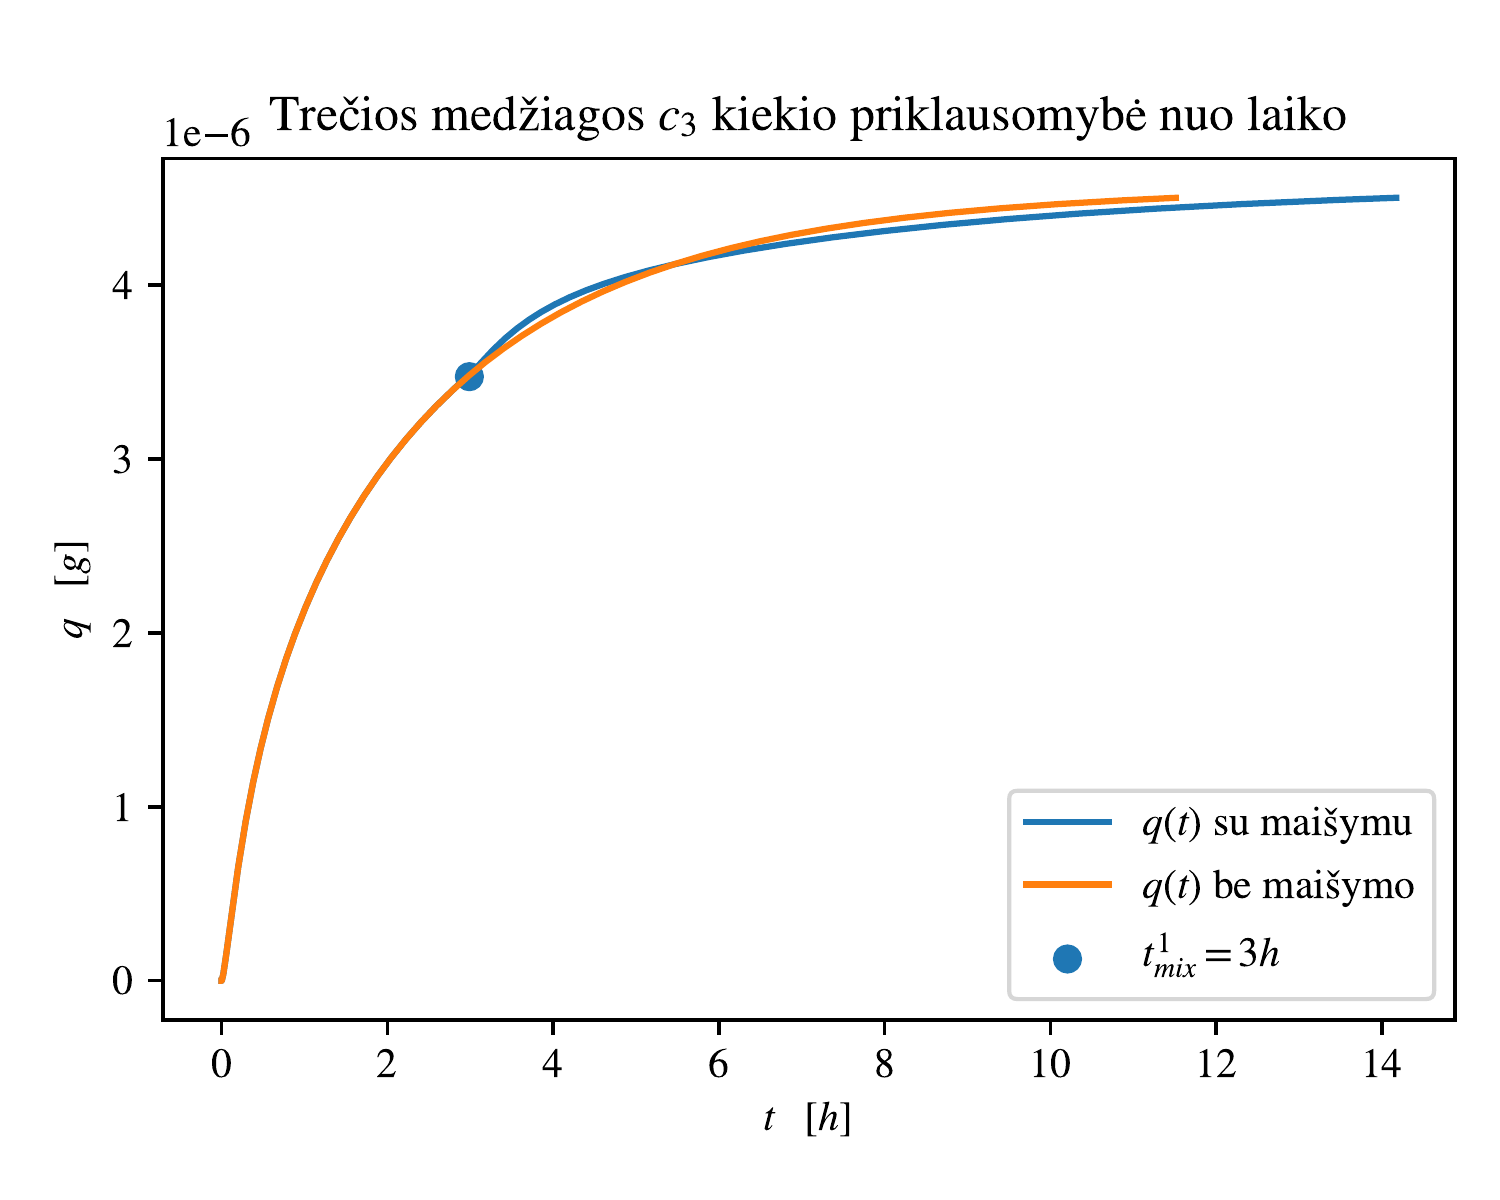
\includegraphics[width=7cm]{paper/assets/bad-mix-qnt-compare-1.png}
        \caption{Atsitiktinio išmaišymo modelio \eqref{random-mix} problema - gali ženkliai prailginti reakcijos pabaigos laiką. Tokio modelio poveiki reikia matuoti statistiniu bandymu arba pilnu perrinkimu. }
    \end{figure}
\end{frame}

\begin{frame}
\frametitle{Tobulas maišymas}
\begin{figure}
\centering
\begin{tikzpicture}[scale=1.5]
    % Original Grid
    \fill[gray!30] (0,1) rectangle (1, 2);
    \fill[gray!30] (1,0) rectangle (2, 1);
    \draw[<->] (0.75,0.75) -- (1.25,1.25);
    \draw[<->] (1.25,0.75) -- (0.75,1.25);
    \draw[thick] (0,0) rectangle (2,2);
    \draw[dashed] (1,0) -- (1,2);
    \draw[dashed] (0,1) -- (2,1);

    \node at (0.5,1.5) {$\Omega_1$};
    \node at (1.5,1.5) {$\Omega_2$};
    \node at (0.5,0.5) {$\Omega_3$};
    \node at (1.5,0.5) {$\Omega_4$};

    % Arrow
    \draw[->, thick] (2.5,1) -- (3.5,1);

    % Transformed Grid
    \begin{scope}[shift={(4,0)}]
        \fill[gray!30] (0,1) rectangle (1, 2);
        \fill[gray!30] (1,0) rectangle (2, 1);
        
        \draw[dashed] (0,0) rectangle (2,2);
        \draw[thick] (1,0) -- (1,2);
        \draw[thick] (0,1) -- (2,1);

        \node at (0.5,1.5) {$\Omega_4$};
        \node at (1.5,1.5) {$\Omega_3$};
        \node at (0.5,0.5) {$\Omega_2$};
        \node at (1.5,0.5) {$\Omega_1$};
    \end{scope}
\end{tikzpicture}
\caption{Tobulo išmaišymo metu metu reakcijos erdvės sritys yra susikeičiamos vietomis įstrižai, tokiu būdu reakcijos greitis padidėja daugiausiai. }
\label{perfect-mix}
\end{figure}
\end{frame}

\begin{frame}
\frametitle{Tobulo maišymo rezultatai}
\begin{figure}
\centering
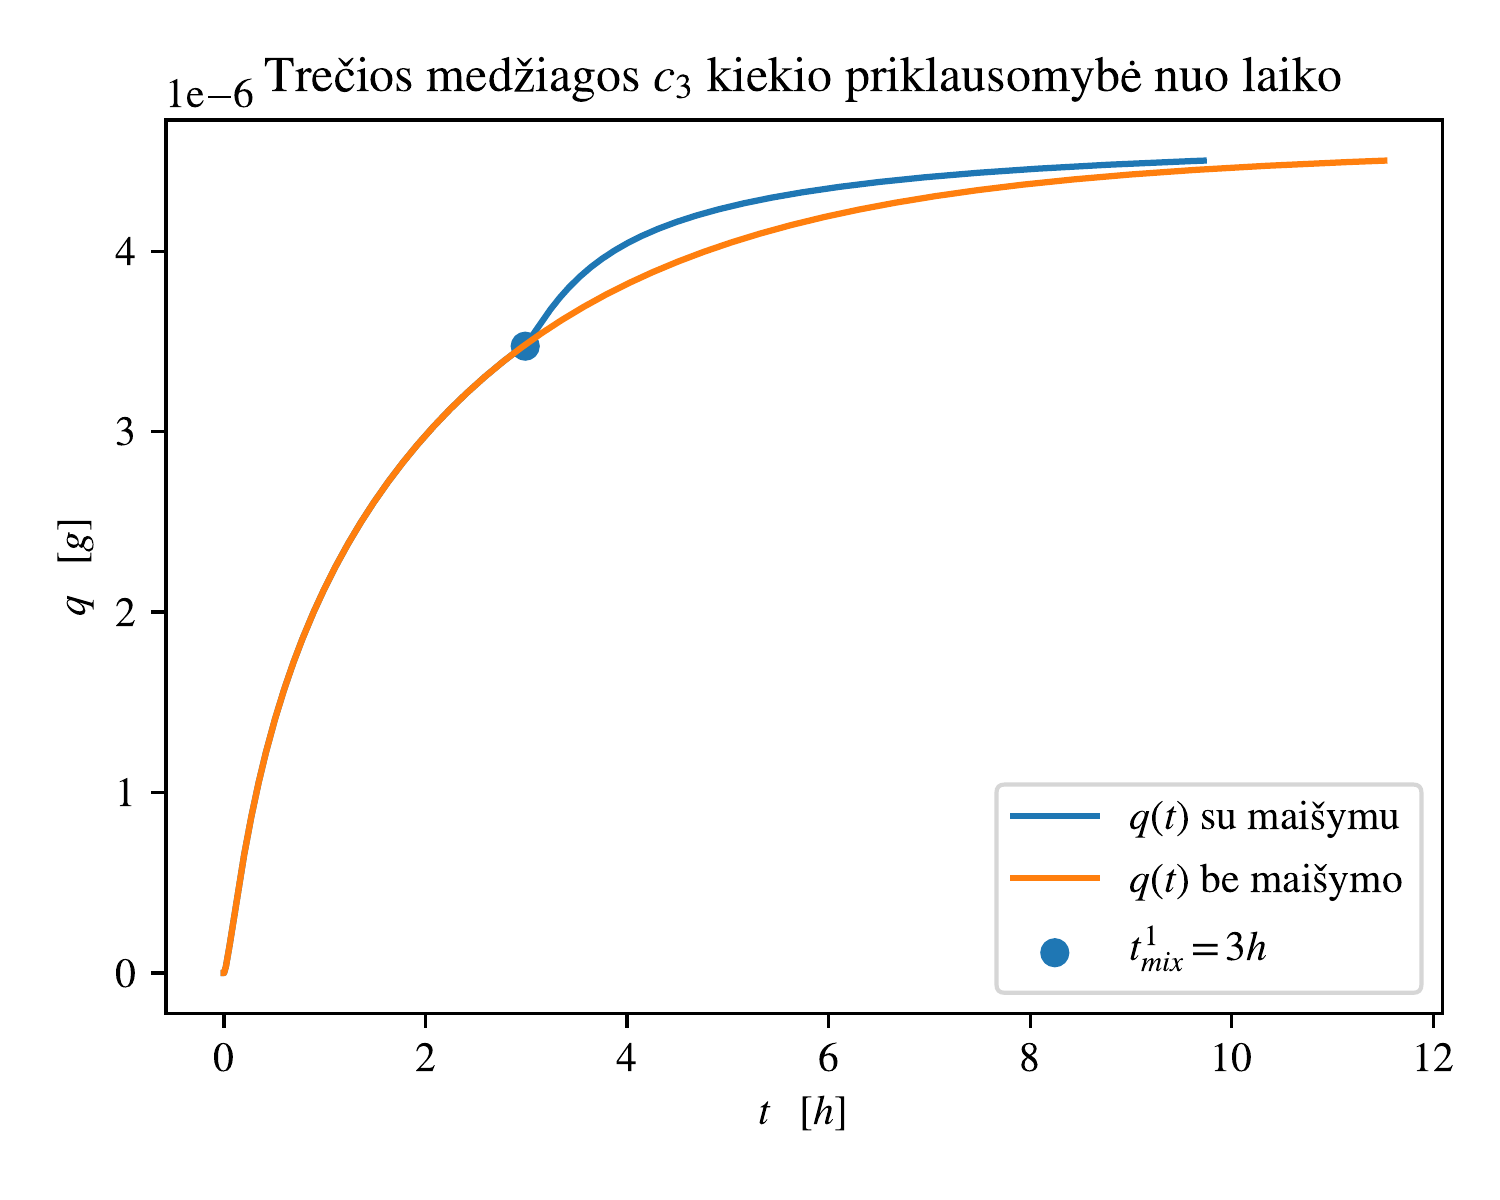
\includegraphics[width=7cm]{paper/assets/optimal-mix-qnt-1.png}
\caption{Tobulas maišymas deterministinis ir tikroviškiau atspindi išmaišymo pasekmes.}
\end{figure}
\end{frame}

\begin{frame}
    \frametitle{Tobulo maišymo rezultatai}
    \begin{figure}
        \centering
        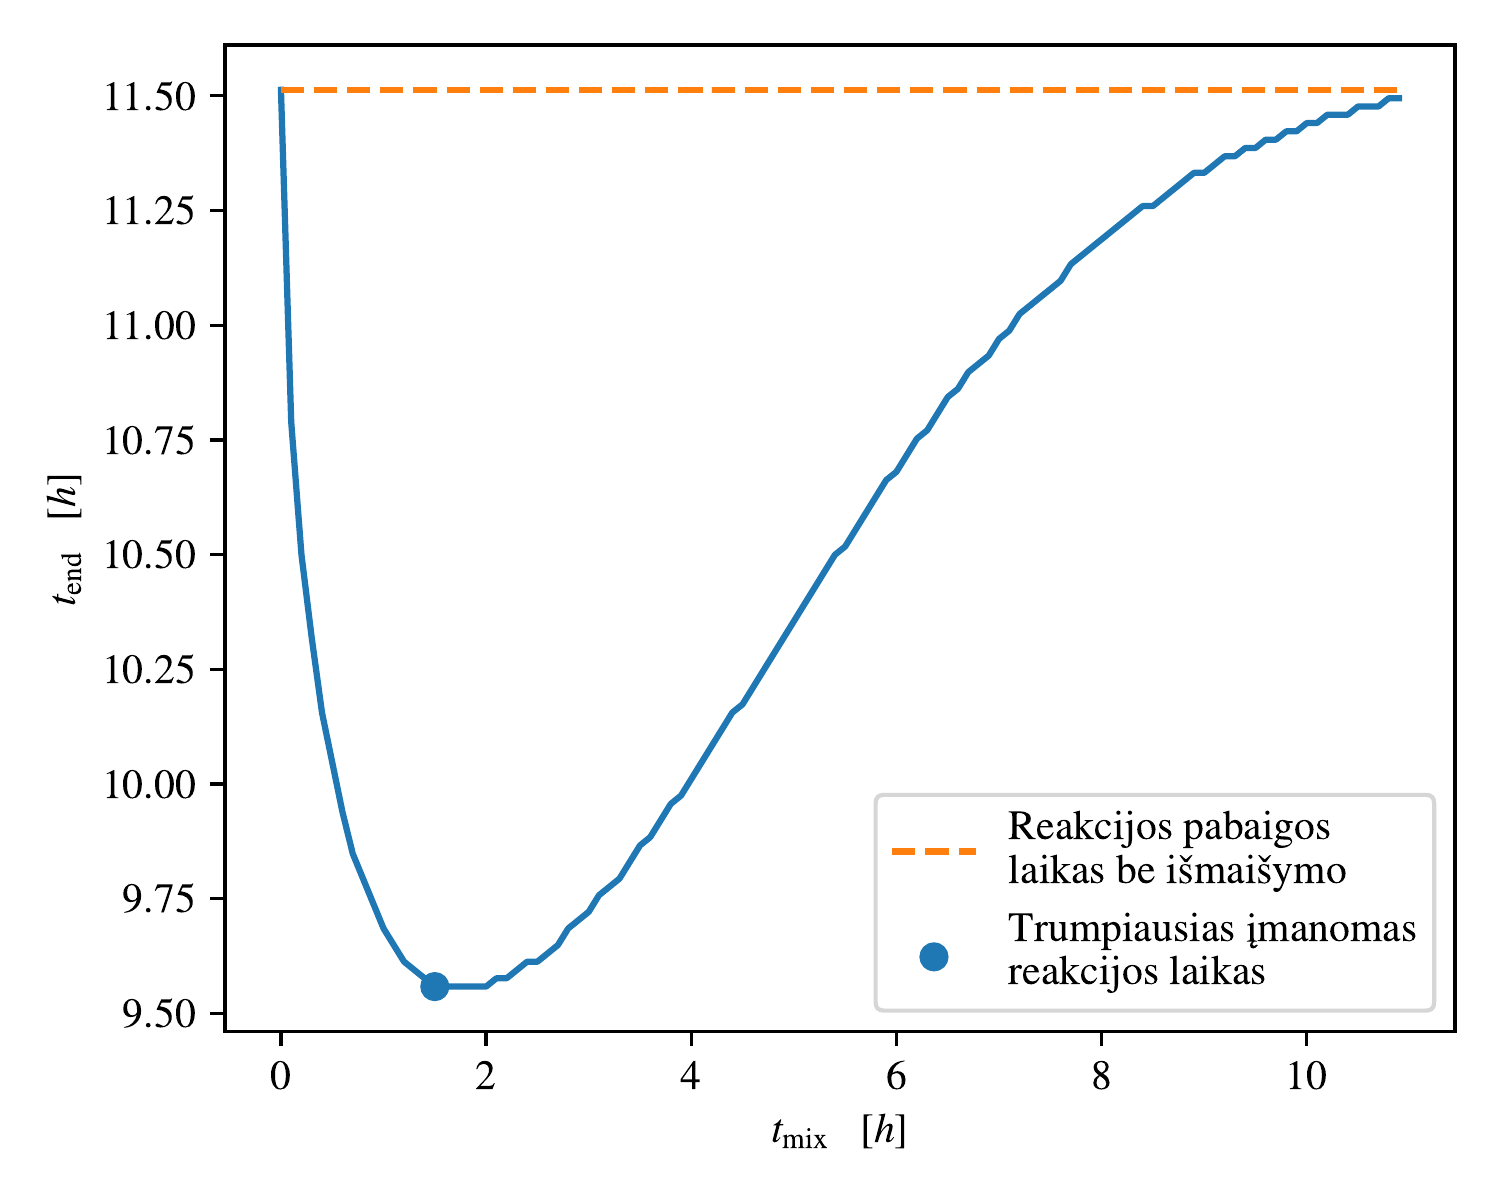
\includegraphics[width=7cm]{paper/assets/mix-end-1.png}
        \caption{Reakcijos pabaigos laiko priklausomybė nuo išmaišymo laiko, kai naudojamas tobulo išmaišymo modelis \eqref{perfect-mix}.}
    \end{figure}
\end{frame}

\begin{frame}
    \frametitle{Maišymas didesnėje erdvėje}
    \begin{figure}
    \centering
    \begin{tikzpicture}
        % Original Grid
    
        \fill[gray!30] (1, 0) rectangle (3, 1);
        \fill[gray!30] (1, 3) rectangle (3, 4);
    
        \fill[gray!30] (0, 1) rectangle (1, 3);
        \fill[gray!30] (3, 1) rectangle (4, 3);
    
        \draw[thick] (0,0) rectangle (2,2);
        \draw[thick] (0,2) rectangle (2,4);
        \draw[thick] (2,0) rectangle (4,2);
        \draw[thick] (2,2) rectangle (4,4);
        \draw[dashed] (1,0) -- (1,4);
        \draw[dashed] (0,1) -- (4,1);
        \draw[dashed] (3,0) -- (3,4);
        \draw[dashed] (0,3) -- (4,3);
    
        \draw[<->] (0.75,0.75) -- (1.25,1.25);
        \draw[<->] (1.25,0.75) -- (0.75,1.25);
    
        \draw[<->] (2.75,0.75) -- (3.25,1.25);
        \draw[<->] (3.25,0.75) -- (2.75,1.25);
    
        \draw[<->] (0.75,2.75) -- (1.25,3.25);
        \draw[<->] (1.25,2.75) -- (0.75,3.25);
    
        \draw[<->] (2.75,2.75) -- (3.25,3.25);
        \draw[<->] (3.25,2.75) -- (2.75,3.25);
    
        \node at (0.5,3.5) {$\Omega_1$};
        \node at (1.5,3.5) {$\Omega_2$};
        \node at (0.5,2.5) {$\Omega_5$};
        \node at (1.5,2.5) {$\Omega_6$};
    
        \node at (2.5,3.5) {$\Omega_3$};
        \node at (3.5,3.5) {$\Omega_4$};
        \node at (2.5,2.5) {$\Omega_7$};
        \node at (3.5,2.5) {$\Omega_8$};
    
        \node at (0.5,1.5) {$\Omega_9$};
        \node at (1.5,1.5) {$\Omega_{10}$};
        \node at (0.5,0.5) {$\Omega_{13}$};
        \node at (1.5,0.5) {$\Omega_{14}$};
    
        \node at (2.5,1.5) {$\Omega_{11}$};
        \node at (3.5,1.5) {$\Omega_{12}$};
        \node at (2.5,0.5) {$\Omega_{15}$};
        \node at (3.5,0.5) {$\Omega_{16}$};
    
        % Arrow
        \draw[->, thick] (4.5,2) -- (5.5,2);
    
        % Transformed Grid
        \begin{scope}[shift={(6,0)}]
            \fill[gray!30] (1, 0) rectangle (3, 1);
            \fill[gray!30] (1, 3) rectangle (3, 4);
    
            \fill[gray!30] (0, 1) rectangle (1, 3);
            \fill[gray!30] (3, 1) rectangle (4, 3);
    
            \draw[dashed] (0,0) rectangle (4,4);
    
            \draw[dashed] (2,0) -- (2,4);
            \draw[dashed] (0,2) -- (4,2);
    
            \draw[thick] (1,0) -- (1,4);
            \draw[thick] (0,1) -- (4,1);
            \draw[thick] (3,0) -- (3,4);
            \draw[thick] (0,3) -- (4,3);
    
            \node at (0.5,3.5) {$\Omega_6$};
            \node at (1.5,3.5) {$\Omega_5$};
            \node at (0.5,2.5) {$\Omega_2$};
            \node at (1.5,2.5) {$\Omega_1$};
    
            \node at (2.5,3.5) {$\Omega_8$};
            \node at (3.5,3.5) {$\Omega_7$};
            \node at (2.5,2.5) {$\Omega_4$};
            \node at (3.5,2.5) {$\Omega_3$};
    
            \node at (0.5,1.5) {$\Omega_{14}$};
            \node at (1.5,1.5) {$\Omega_{13}$};
            \node at (0.5,0.5) {$\Omega_{10}$};
            \node at (1.5,0.5) {$\Omega_{9}$};
    
            \node at (2.5,1.5) {$\Omega_{16}$};
            \node at (3.5,1.5) {$\Omega_{15}$};
            \node at (2.5,0.5) {$\Omega_{12}$};
            \node at (3.5,0.5) {$\Omega_{11}$};
        \end{scope}
    \end{tikzpicture}
    \caption{Tobulo maišymo modelis didesnėje erdvėje analogiškas modeliui \eqref{perfect-mix} atkartojant jį periodiškai.}
    \label{large-perfect-mix}
\end{figure}
\end{frame}

\begin{frame}
    \frametitle{Maišymas didesnėje erdvėje}
    \begin{figure}
    \centering
    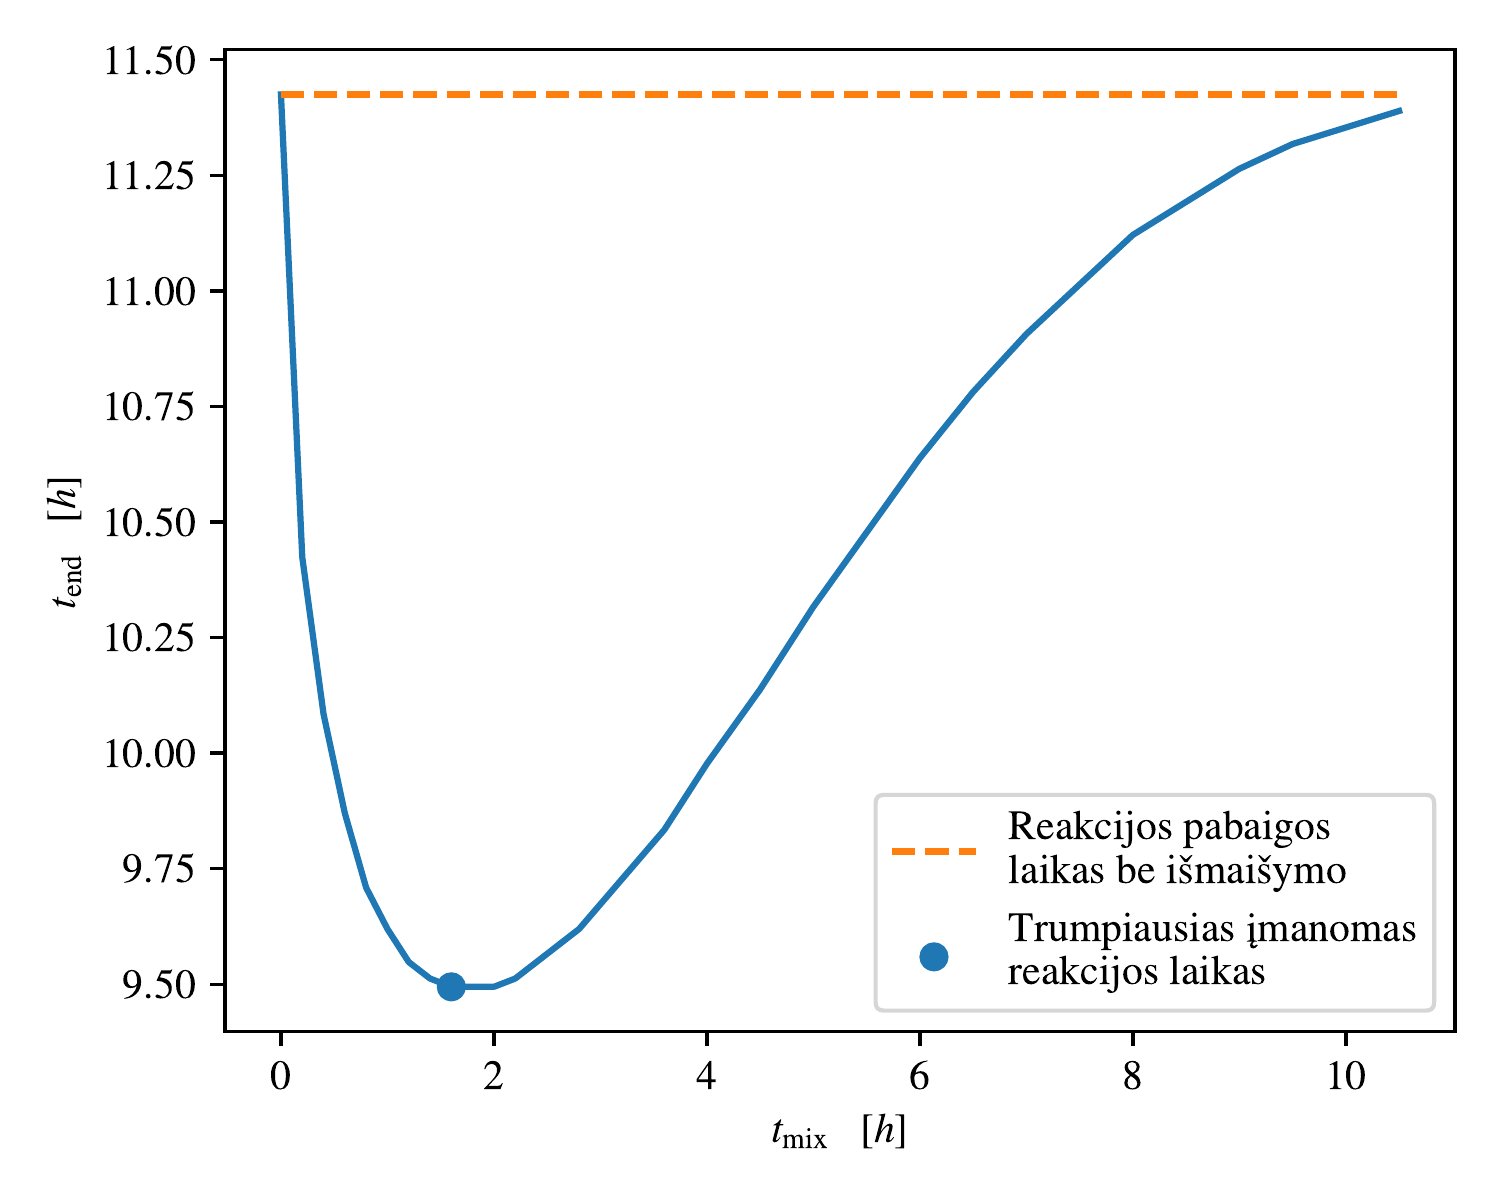
\includegraphics[width=7cm]{paper/assets/mix-end-large-1.png}
    \caption{Reakcijos pabaigos laiko priklausomybė nuo išmaišymo laiko, kai naudojamas tobulo išmaišymo modelis didesnėje erdvėje \eqref{large-perfect-mix}.}
    \end{figure}
\end{frame}

\begin{frame}
\frametitle{Rezultatai}
\begin{itemize}
    \item Sukurtas kompiuterinis YAG reakcijos modelis. 
    \item Teoriškai parodyta skaitinio modelio stabilumo sąlyga
    \item Kompiuterinio modelio rezultatai buvo analizuojami ir buvo užtikrinta, kad modelis veikia korektiškai
    \item Pasiūlyti du maišymo modeliai - atsitiktinis ir tobulas
    \item Išmaišymo modeliai integruoti į kompiuterinį YAG reakcijos modelį
    \item Atlikta papildyto kompiuterinio modelio rezultatų analizė
\end{itemize}
\end{frame}

\begin{frame}
\frametitle{Išvados}
\begin{itemize}
    \item Atsitiktinio maišymo modelio rezultatai neatitinka realybėje pastebimų rezultatų, kai reakcija modeliuojama mažoje srityje, kurioje susiduria tik 4-ios mikrodalelės. Norint iš šio modelio išgauti tikrovę atitinkančius rezultatus yra būtina modeliuoti didesnę erdvės sritį.

    \item Tobulo išmaišymo modelio rezultatai atitinka realybėje pastebimą reakcijos pagreitėjimą.
    
    \item Modeliuojant didesnę erdvės sritį, tobulo išmaišymo modelio rezultatai kinta gana nežymiai, todėl maišymo modeliavimui užtenka modeliuoti mažą reakcijos erdvės sritį su 4-iom skirtingų medžiagų mikrodalelėmis

\end{itemize}
\end{frame}

\begin{frame}
\frametitle{Literatūros šaltiniai}
\printbibliography
\end{frame}

\end{document}